\documentclass[10pt]{beamer}
\usepackage[utf8]{inputenc}

\usetheme{Madrid}
\usecolortheme{default}
\usepackage{graphicx}
\usepackage{amsmath}
\usepackage{booktabs}
\usepackage{amsmath,amssymb,amsthm,microtype}
\usepackage{tikz}
\graphicspath{{../OverleafPaper/figures/}{OverleafPaper/figures/}{../forgetting/outputs/test/monte_carlo/figures/}{forgetting/outputs/test/monte_carlo/figures/}{../forgetting/outputs/test/first_2000/figures/individual_states/p0_0.5/}{forgetting/outputs/test/first_2000/figures/individual_states/p0_0.5/}{../forgetting/outputs/test/first_2000/figures/state_distributions/p0_0.5/}{forgetting/outputs/test/first_2000/figures/state_distributions/p0_0.5/}}

\title{Weekly report}
\author{Natalia Trigo Tomasevich}
\date{\today}

\begin{document}

\frame{\titlepage}

\begin{frame}{From last week}
    \begin{itemize}[<+->]
        \item Complete proof of the fluid model result
        \item Exploration of the competition model 
        \item Insights about the parameters of the problem 
    \end{itemize}
\end{frame}

\begin{frame}{Fluid approximation}
    Recall the state dynamics
    \begin{equation}
        \dot x(t)=D(x(t))\lambda(p_{i(t)}-x(t))
    \end{equation}
    and the provider's problem 
    \begin{equation}\label{eq:fluid-value}
        V(x)=\sup\int_0^\infty e^{-\delta t}D(x(t))(R-c_{i(t)})\,dt,
        \qquad x(0)=x.
    \end{equation}
    \pause
    The problem with this equation is that the instantaneous payoff are dependent on the product choice. Can we transform the problem so that the two products have the same payoff and differ only on how they move the state? 
\end{frame}

\begin{frame}{Transforming the problem}
    We start from the HJB equation for the fluid model
    \begin{equation}\label{eq:fluid-HJB}
        \delta V(x)=D(x)\max_{i\in\{1,2\}}
        \{R-c_i+\lambda(p_i-x)V'(x)\}.
    \end{equation}
    Comparing product 2 vs product 1 we get
    \begin{equation*}
        i=2 \quad \iff \quad V'(x)>\frac{\Delta c}{\lambda\Delta p}
    \end{equation*}
\end{frame}

\begin{frame}{Transforming the problem}
    Product 2 has an additional instrantaneous cost 
    \begin{equation*}
        D(x)\Delta c 
    \end{equation*}
    But it also increases the drift of the state by 
    \begin{equation*}
        \dot x_2 - \dot x_1 = \lambda(p_2-p_1) = \lambda\Delta p
    \end{equation*}
    Therefore, 
    \begin{equation*}
        \frac{\text{extra cost}}{\text{extra drift}} = \frac{D(x)\Delta c}{\lambda D(x) \Delta p} = \frac{\Delta c}{\lambda\Delta p}
    \end{equation*}
    This ratio does not depend on the state. The additional cost per additional unit of state drift is constant. So we can assign a value of $\frac{\Delta c}{\lambda\Delta p}$ to each unif of state accumulation. Once we do that, the cost difference between the products disappears. 
\end{frame}

\begin{frame}{Transforming the problem}
    Adding $\frac{\Delta c}{\lambda\Delta p}$ to the flow payoff and using the dynamics $\dot x = D(x)\lambda(p_i - x)$ we get
    \begin{align*}
        D(x)(R-c_i)+\frac{\Delta c}{\lambda\Delta p}\dot x
        &=D(x)\left[R-c_i+\frac{\Delta c}{\Delta p}(p_i-x)\right]\\
        &=D(x)\left[R-c_1+\frac{\Delta c}{\Delta p}(p_1-x)\right]
    \end{align*}
    So we have 
    \begin{equation*}
        \Rightarrow D(x)(R-c_i) =D(x)\left[R-c_1+\frac{\Delta c}{\Delta p}(p_1-x)\right] -\frac{\Delta c}{\lambda\Delta p}\dot x
    \end{equation*}
    The first term does not depend ont the product choice.
\end{frame}


\begin{frame}{Transforming the problem}
    Replacing this in the fluid model equation we get
    \begin{equation*}
        V(x) = \sup_{i(\cdot)} \int_{0}^{\infty} e^{-\delta t}\left[D(x(t))\left(R-c_1 + \frac{\Delta c}{\Delta p}(p_1-x(t))\right)-\frac{\Delta c}{\lambda\Delta p}\dot x(t)\right]dt
    \end{equation*} 
    Integrating by parts and doing more math we get
    \begin{equation}
        V(x) = \frac{\Delta c}{\lambda\Delta p} x + \sup_{i(\cdot)} \int_{0}^{\infty} e^{-\delta t} F(x(t))dt
    \end{equation} 
    Where 
    \begin{equation*}
        F(x) = D(x)\left(R-c_1 + \frac{\Delta c}{\Delta p}(p_1-x)\right)-\frac{\delta\Delta c}{\lambda\Delta p}x
    \end{equation*}
\end{frame}

\begin{frame}{Why is this transformation useful?}
    We can define 
    \begin{equation*}
        W(x) = V(x) - \frac{\Delta c}{\lambda \Delta p}x \quad \Rightarrow \quad V'(x) = W'(x) + \frac{\Delta c}{\lambda \Delta p}
    \end{equation*}
    \pause
    So our condition becomes
    \begin{equation*}
          V'(x) > \frac{\Delta c}{\lambda \Delta p} \quad \iff \quad W'(x) > 0
    \end{equation*}
    \pause
    and the transformed HJB is 
    \begin{equation}
        \delta W(x) = F(x) + \max_{i} \{ \lambda D(x)(p_i - x) \}
    \end{equation}
    \pause
    Now both products face the same payoff $F(x)$ and they differ only in how they move the state.
\end{frame}

\begin{frame}{What we want to prove}
    \begin{block}{Proposition}
        The fluid problem admits an optimal stationary policy with numbers
        $0\le x_L\le x_H\le1$ such that, away from threshold states,
        \begin{equation*}
        i(x)=
        \begin{cases}
        1,&x<x_L,\\
        2,&x_L<x<x_H,\\
        1,&x>x_H.
        \end{cases}
        \end{equation*}
    \end{block}
    \pause
    This is equivalent to proving that $\{x \in [0,1] : W'(x) >0\}$ is an interval or that we can only see the patterns $1\rightarrow2$, $2\rightarrow1$, $1\rightarrow2\rightarrow1$ or constant policies but NOT $1\rightarrow2\rightarrow1\rightarrow2$.
\end{frame}

\begin{frame}{How do we prove it}
    We first study the shape of $F$ and then we use the HJB to restrict the shape of $W$. Define 

    \begin{equation*}
        g(x) = \delta W(x) -F(x) = \max_i \{b_i(x)W'(x)\}
    \end{equation*}
    where 
    \begin{equation*}
        b_i(x) = \lambda D(x)(p_i - x) \qquad \text{(Drifts)}
    \end{equation*}
    \pause
    On a region were product $i$ is being used we have
    \begin{equation*}
        g(x) = b_i(x)W'(x) \quad \Rightarrow \quad W'(x) = \frac{g(x)}{b_i(x)}
    \end{equation*}
    \pause
    differentiating this with respect to $x$ we get
    \begin{equation*}
        g'(x) =  \delta W'(x) -F'(x) = \frac{\delta}{b_i(x)}g(x) - F'(x)
    \end{equation*}
\end{frame}

\begin{frame}{Connection between $W$ and $F$}
    Consider $x^*$ away from $p_1$ and $p_2$ such that $W'(x^*) = 0$. Then,
    $$g(x^*) = b_i(x^*)W'(x^*) = 0$$ \pause
    since $b_i(x^*) \neq 0$,
    $$g'(x^*) = \frac{\delta}{b_i(x^*)}g(x^*) - F'(x^*) = -F'(x^*)$$
    So at a possible switching point, the sign of $F'$ tells us the direction in which $g$ can cross zero.
\end{frame}

\begin{frame}{Lemma}
    \begin{block}{Lemma}
        The set $\{x\in[0,1]:F'(x)>0\}$ is an interval, possibly empty or
        meeting a boundary. If nonempty, $F$ decreases before this interval,
        increases within it, and decreases after it, with absent segments omitted.
        If it is empty, product 1 is optimal everywhere.
    \end{block}
    This proof is in the progress notes.
\end{frame}

\begin{frame}{What we want to prove now}
    \begin{block}{Proposition}
        Suppose $0<p_1<p_2<1$, and $\delta,\lambda>0$.
        Allow relaxed controls, so that any state in $[p_1,p_2]$ can be held fixed.
        Suppose that, for some $0\leq a<m\leq 1$,
        \begin{equation}
            F'(x)<0 \quad \text{on } (0,a)\cup(m,1),
            \qquad
            F'(x)>0 \quad \text{on } (a,m),
        \end{equation}
        with any interior zeros of $F'$ being simple. Then an optimal policy can be
        selected which uses product 2 on at most one interval and product 1 outside it.
        Thus, as the state increases, the only nonconstant action patterns are
        \begin{equation}
            1\to2,\qquad 2\to1,\qquad 1\to2\to1.
        \end{equation}
    \end{block}
\end{frame}
\begin{frame}
    \frametitle{Proof}
    First we notice that the sign of the drifts $b_i(x)$ is determined by the position of $x$:
    \begin{align}
        b_1(x) &>0 \,,\quad b_2(x)>0 \quad \text{for } x<p_1 \\
        b_1(x) &<0 \,,\quad b_2(x)>0 \quad \text{for } p_1< x <p_2 \\
        b_1(x) &<0 \,,\quad b_2(x)<0 \quad \text{for } x > p_2  
    \end{align} 

    Since $g = b_i W'$ for any branch of product $i$, we have that the sign of $g$ is related to the sign of $W'$, specifically:
    \begin{align}
        \text{sign}(g) &= \text{sign}(W') \,,\,\,\,\,\,\quad \text{for } x<p_1 \\
        \text{sign}(g) &= -\text{sign}(W') \,,\quad \text{for } x>p_2
    \end{align} 
\end{frame}

\begin{frame}
    \frametitle{Outside $[p_1,p_2]$}
    At an interior zero of $g$ with $F'\ne0$, we have that $g' = -F'$, so  
    \begin{equation*}
        \begin{array}{c|cc}
        &F'<0&F'>0\\ \hline
        x<p_1&1\to2&2\to1\\
        x>p_2&2\to1&1\to2.
        \end{array}
        \tag{*}
    \end{equation*} 
    The case where $F'=0$ is not a problem because $F'$ has simple zeros, when this happens and $g=0$, it does without changing sign.
\end{frame}


\begin{frame}
    \frametitle{Inside $[p_1,p_2]$}
    \begin{itemize}[<+->]
    \item Consider the case $m>p_1$ and define $h= min\{m,p_2\}$
    \item In this region we have that 
    $$b_1(x)<0<b_2(x)$$
    \item Product 1 moves the state towards $p_1$ and product 2 moves it towards $p_2$
    \item We define $L(x)$ as the value of moving towards $p_1$ and $H(x)$ as the value of moving towards $h$. They satisfy the Bellman equations: $$\delta L = F + b_1L' \qquad \delta H = F + b_2H'$$
    \item On the decreasing part of $F$,moving left toward $p_1$ raises the future flow payoff. On the increasing part, moving right toward $p_2$ does the same.
    \end{itemize}
\end{frame}

\begin{frame}
    \frametitle{Inside $[p_1,p_2]$}
    \begin{itemize}[<+->]
        \item That gives us $$\delta \max\{L(x),H(x)\}>F(x)$$
        \item If $L$ wins because of $b_1(x)<0<b_2(x)  $ we have that $L'<0$
        \item If $H$ wins because of $b_1(x)<0<b_2(x)  $ we have that $H'>0$
        \item Then, considering an interior crossing $x^*\in(p_1,h)$ such that $L(x^*)=H(x^*)$, we have that $$\delta L(x^*)-F(x^*) = \delta H(x^*)-F(x^*) >0 $$ and with $b_1(x^*)<0<b_2(x^*)$ we have $$L'(x^*) = \frac{\delta L (x^*) - F(x^*)}{b_1(x^*)}<0 ,\qquad H'(x^*) = \frac{\delta H (x^*) - F(x^*)}{b_2(x^*)}>0$$
        \item Then $(H-L)'(x^*)>0$, which means that $H$ wins immediately to the right of $x^*$ and $L$ wins immediately to the left.
    \end{itemize}
    
\end{frame}

\begin{frame}
    \frametitle{Inside $[p_1,p_2]$}
    \begin{itemize}
        \item The second part of this case is to prove that the maximum of $L$ and $H$ is the optimal policy, that I won't show here but you can find in the progress notes.
        \item With this we have that if there is any crossing it must be unique and going from $L$ to $H$.
    \end{itemize}
    \pause
    \begin{figure}[H]
    \centering
    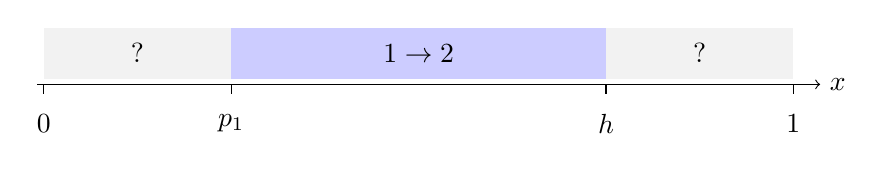
\begin{tikzpicture}[x=0.68cm,y=1cm]
    \fill[gray!10] (0,0.07) rectangle (3.5,0.72);
    \fill[blue!20] (3.5,0.07) rectangle (10.5,0.72);
    \fill[gray!10] (10.5,0.07) rectangle (14,0.72);
    \node at (1.75,0.395) {$?$};
    \node at (7,0.395) {$1\to2$};
    \node at (12.25,0.395) {$?$};
    \draw[->] (-0.12,0) -- (14.5,0) node[right] {$x$};
    \foreach \x/\lab in {0/0,3.5/p_1,10.5/h,14/1} {
    \draw (\x,0) -- (\x,-0.12);
    \node[below=4pt] at (\x,-0.12) {$\lab$};
    }
    \end{tikzpicture}
    \label{fig:middle-interval-policy}
    \end{figure}
\end{frame}

% \begin{frame}
%     \frametitle{When $m\le p_1$}
%         \begin{figure}[H]
%         \centering
%         \begin{minipage}{\textwidth}
%         \centering
%         \textbf{(a) $x\ge m$}\par\smallskip
%         \begin{tikzpicture}[x=1cm,y=1cm]
%         \fill[blue!20] (1,-0.13) rectangle (5,0.13);
%         \draw[->] (-0.35,0) -- (5.45,0) node[right] {$x$};
%         \foreach \x/\lab in {0/0,1/m,2.2/p_1,3.8/p_2,5/1} {
%         \draw (\x,-0.08) -- (\x,0.08);
%         \node[above=4pt] at (\x,0.08) {$\lab$};
%         }
%         \fill (1,0) circle (1.8pt);
%         \end{tikzpicture}
%         \end{minipage}\par\vspace{0.9cm}
%         \begin{minipage}{\textwidth}
%         \centering
%         \textbf{(b) $x<m$}\par\smallskip
%         \begin{tikzpicture}[x=1cm,y=1cm]
%         \fill[blue!20] (0,-0.13) rectangle (1,0.13);
%         \draw[->] (-0.35,0) -- (5.45,0) node[right] {$x$};
%         \foreach \x/\lab in {0/0,1/m,2.2/p_1,3.8/p_2,5/1} {
%         \draw (\x,-0.08) -- (\x,0.08);
%         \node[above=4pt] at (\x,0.08) {$\lab$};
%         }
%         \draw[fill=white] (1,0) circle (1.8pt);
%         \end{tikzpicture}
%         \end{minipage}
%         \end{figure}
% \end{frame}

\begin{frame}
    \frametitle{When $m\le p_1$ }
    \begin{itemize}
        \item From any state $x\ge0$ no product can move the state below $m$ and since $F$ is decreasing above $m$, product 1 generates the smallest trajectory so it is optimal
        \item Below $m$ we have $x<p_1$ so from the crossing table we have at most $1\rightarrow2$ when $F$ is decreasing and $2 \to 1$ when $F$ is increasing.
    \end{itemize}

    Then we have 

    \begin{figure}[H]
    \centering
    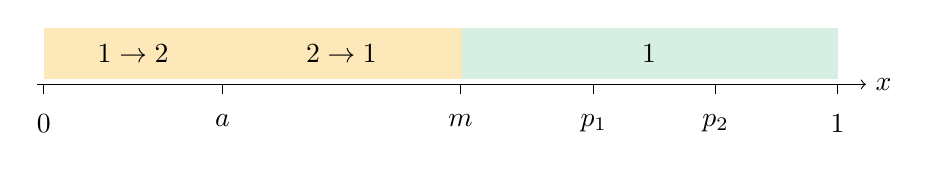
\begin{tikzpicture}[x=0.72cm,y=1cm]
    \definecolor{policyStart}{HTML}{FCE8B8}
    \definecolor{policyEnd}{HTML}{FCE8B8}
    \definecolor{policyHold}{HTML}{D7EEE2}
    \fill[policyStart] (0,0.07) rectangle (3.15,0.72);
    \fill[policyEnd] (3.15,0.07) rectangle (7.35,0.72);
    \fill[policyHold] (7.35,0.07) rectangle (14,0.72);
    \node at (1.575,0.395) {$1\to2$};
    \node at (5.25,0.395) {$2\to1$};
    \node at (10.675,0.395) {$1$};
    \draw[->] (-0.12,0) -- (14.5,0) node[right] {$x$};
    \foreach \x/\lab in {0/0,3.15/a,7.35/m,9.7/p_1,11.85/p_2,14/1} {
    \draw (\x,0) -- (\x,-0.12);
    \node[below=4pt] at (\x,-0.12) {$\lab$};
    }
    \end{tikzpicture}
    \end{figure}

\end{frame}

\begin{frame}
    \frametitle{When $p_1<m\le p_2$}
    \begin{itemize}
        \item For $x>m$ we want to go back to $m$ and since $b_1(x)<b_2(x)$ at every state, the trajectory generated by poduct 1 is smaller than any other trajectory. Hence, product 1 is optimal
        \item On $[p_1,m]$ we already saw that the only crossing that can exists is $1\rightarrow2$ (case h=m)
    \end{itemize}
    With these results we have 
    \begin{figure}[H]
    \centering
    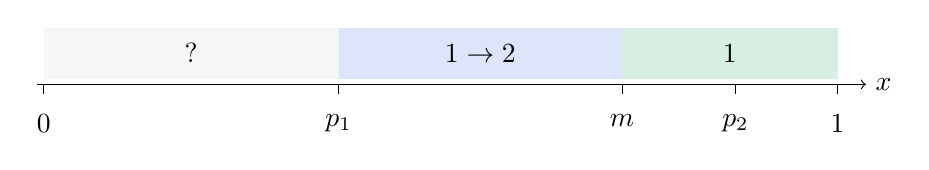
\begin{tikzpicture}[x=0.72cm,y=1cm]
    \definecolor{policyUnknown}{HTML}{F5F6F7}
    \definecolor{policyComparison}{HTML}{DDE5FA}
    \definecolor{policyHold}{HTML}{D7EEE2}
    \fill[policyUnknown] (0,0.07) rectangle (5.2,0.72);
    \fill[policyComparison] (5.2,0.07) rectangle (10.2,0.72);
    \fill[policyHold] (10.2,0.07) rectangle (14,0.72);
    \node at (2.6,0.395) {$?$};
    \node at (7.7,0.395) {$1\to2$};
    \node at (12.1,0.395) {$1$};
    \draw[->] (-0.12,0) -- (14.5,0) node[right] {$x$};
    \foreach \x/\lab in {0/0,5.2/p_1,10.2/m,12.2/p_2,14/1} {
        \draw (\x,0) -- (\x,-0.12);
        \node[below=4pt] at (\x,-0.12) {$\lab$};
    }
    \end{tikzpicture}
    \end{figure}
\end{frame}

\begin{frame}
    \frametitle{When $p_1<m\le p_2$}
    When $a>p_1$ and $L$ wins at $p_1$
    \begin{itemize}
        \item Below $p_1$ we have $F'<0$ so the only possible crossing is $1\to2$
        \item Here $W(p_1)=L(p_1) = F(p_1)/\delta \rightarrow g(p_1) =0$
        \item A contradiction argument shows that product 1 must be optimal immediately to the left of $p_1$
        \item A product 2 region below $p_1$ would require a $2 \to 1$ crossing and that is not allowed
    \end{itemize}
    \begin{figure}[H]
    \centering
    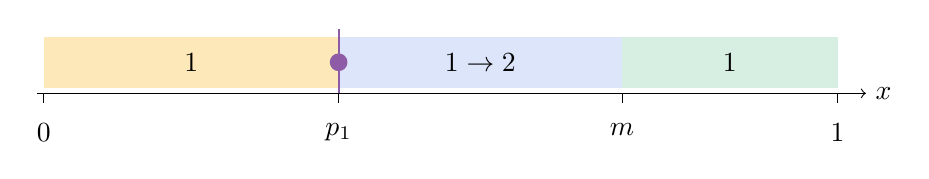
\begin{tikzpicture}[x=0.72cm,y=1cm]
    \definecolor{policyLow}{HTML}{FCE8B8}
    \definecolor{policyComparison}{HTML}{DDE5FA}
    \definecolor{policyHold}{HTML}{D7EEE2}
    \definecolor{policyBoundary}{HTML}{8E5BA6}
    \fill[policyLow] (0,0.07) rectangle (5.2,0.72);
    \fill[policyComparison] (5.2,0.07) rectangle (10.2,0.72);
    \fill[policyHold] (10.2,0.07) rectangle (14,0.72);
    \draw[policyBoundary,line width=0.8pt] (5.2,0) -- (5.2,0.82);
    \fill[policyBoundary] (5.2,0.395) circle (3.2pt);
    \node at (2.6,0.395) {$1$};
    \node at (7.7,0.395) {$1\to2$};
    \node at (12.1,0.395) {$1$};
    \draw[->] (-0.12,0) -- (14.5,0) node[right] {$x$};
    \foreach \x/\lab in {0/0,5.2/p_1,10.2/m,14/1} {
        \draw (\x,0) -- (\x,-0.12);
        \node[below=4pt] at (\x,-0.12) {$\lab$};
    }
    \end{tikzpicture}
    \end{figure}
\end{frame}

\begin{frame}
    \frametitle{When $p_1<m\le p_2$}
    When $a>p_1$ and $H$ wins at $p_1$
    \begin{itemize}
        \item Here we have $W(p_1)=H(p_1) > L(p_1) = F(p_1)/\delta$
        \item Then $g(p_1) > 0$ and by continuity, $g(x) > 0$ to the left of $p_1$
        \item Since $0<b_1(x)<b_2(x)$, $W'>0$, hence  product 2 is optimal to the left of $p_1$
        \item Again, the table allows crossing from $1 \to 2$ only so any product 2 region on the left can begin at most once and must continue up to $p_1$
    \end{itemize}
    \begin{figure}[H]
    \centering
    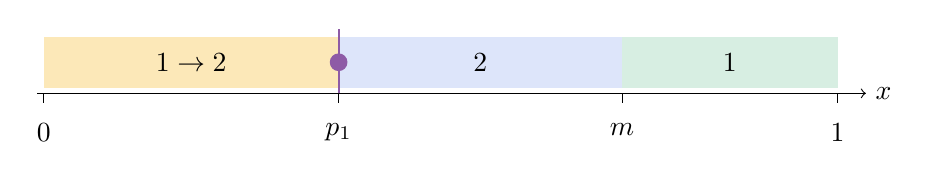
\begin{tikzpicture}[x=0.72cm,y=1cm]
    \definecolor{policyLow}{HTML}{FCE8B8}
    \definecolor{policyComparison}{HTML}{DDE5FA}
    \definecolor{policyHold}{HTML}{D7EEE2}
    \definecolor{policyBoundary}{HTML}{8E5BA6}
    \fill[policyLow] (0,0.07) rectangle (5.2,0.72);
    \fill[policyComparison] (5.2,0.07) rectangle (10.2,0.72);
    \fill[policyHold] (10.2,0.07) rectangle (14,0.72);
    \draw[policyBoundary,line width=0.8pt] (5.2,0) -- (5.2,0.82);
    \fill[policyBoundary] (5.2,0.395) circle (3.2pt);
    \node at (2.6,0.395) {$1\to2$};
    \node at (7.7,0.395) {$2$};
    \node at (12.1,0.395) {$1$};
    \draw[->] (-0.12,0) -- (14.5,0) node[right] {$x$};
    \foreach \x/\lab in {0/0,5.2/p_1,10.2/m,14/1} {
        \draw (\x,0) -- (\x,-0.12);
        \node[below=4pt] at (\x,-0.12) {$\lab$};
    }
    \end{tikzpicture}
    \end{figure}
\end{frame}

\begin{frame}
    \frametitle{When $p_1<m\le p_2$}
    When $a<p_1$
    \begin{itemize}
        \item On $(a,p_1)$, we have $F'>0$ so moving toward $p_1$ under product 1 raises the future payoff, so $L>F/\delta$ and hence $g>0$
        \item Since $0<b_1(x)<b_2(x)$ we have $W'>0$ and hence product 2 is optimal.
        \item On $(0,a)$, $F'<0$ so only $1 \to 2$ crossing is allowed
        \item Therefore any product 2 region below $a$ must attach to the one on $(a,p_1)$
    \end{itemize}

    \begin{figure}[H]
    \centering
    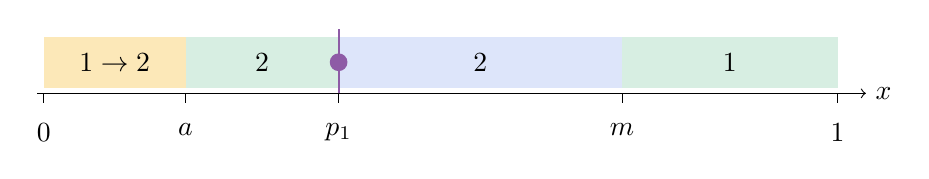
\begin{tikzpicture}[x=0.72cm,y=1cm]
    \definecolor{policyLow}{HTML}{FCE8B8}
    \definecolor{policyComparison}{HTML}{DDE5FA}
    \definecolor{policyHold}{HTML}{D7EEE2}
    \definecolor{policyBoundary}{HTML}{8E5BA6}
    \fill[policyLow] (0,0.07) rectangle (2.5,0.72);
    \fill[policyHold] (2.5,0.07) rectangle (5.2,0.72);
    \fill[policyComparison] (5.2,0.07) rectangle (10.2,0.72);
    \fill[policyHold] (10.2,0.07) rectangle (14,0.72);
    \draw[policyBoundary,line width=0.8pt] (5.2,0) -- (5.2,0.82);
    \fill[policyBoundary] (5.2,0.395) circle (3.2pt);
    \node at (1.25,0.395) {$1\to2$};
    \node at (3.85,0.395) {$2$};
    \node at (7.7,0.395) {$2$};
    \node at (12.1,0.395) {$1$};
    \draw[->] (-0.12,0) -- (14.5,0) node[right] {$x$};
    \foreach \x/\lab in {0/0,2.5/a,5.2/p_1,10.2/m,14/1} {
        \draw (\x,0) -- (\x,-0.12);
        \node[below=4pt] at (\x,-0.12) {$\lab$};
    }
    \end{tikzpicture}
    \end{figure}

\end{frame}

\begin{frame}
    \frametitle{When $p_1<m\le p_2$}
    When $a=p_1$
    \begin{itemize}
        \item $a$ is the valley of $F$
        \item Moving toward the higher destination yields a larger future payoff
        \item Hence, the high branch wins at $p_1$ and by continuity, product 2 is optimal to the left of $p_1$
        \item Since $F'<0$ below $p_1$ the table shows the only possible crossing is $1\to2$
    \end{itemize}
    \begin{figure}[H]
    \centering
    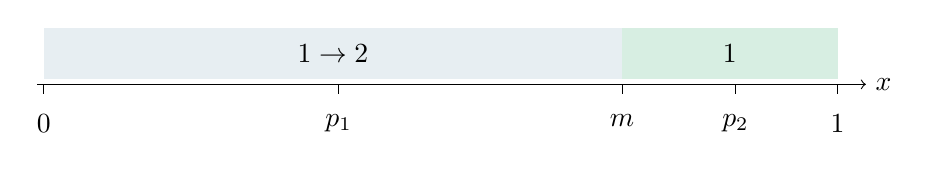
\begin{tikzpicture}[x=0.72cm,y=1cm]
    \definecolor{policyJoined}{HTML}{E7EEF2}
    \definecolor{policyHold}{HTML}{D7EEE2}
    \fill[policyJoined] (0,0.07) rectangle (10.2,0.72);
    \fill[policyHold] (10.2,0.07) rectangle (14,0.72);
    \node at (5.1,0.395) {$1\to2$};
    \node at (12.1,0.395) {$1$};
    \draw[->] (-0.12,0) -- (14.5,0) node[right] {$x$};
    \foreach \x/\lab in {0/0,5.2/p_1,10.2/m,12.2/p_2,14/1} {
        \draw (\x,0) -- (\x,-0.12);
        \node[below=4pt] at (\x,-0.12) {$\lab$};
    }
    \end{tikzpicture}
    \end{figure}
\end{frame}

\begin{frame}
    \frametitle{When $m>p_2$}
    \begin{itemize}
        \item In $[p_1,p_2]$ the destination comparison is straightforward
        \item Below $p_1$ we also saw it already
        \item If $a\ge p_2$, any trajectory starting at $x<a$ remains below $a$ and product 1 is optimal
        \item For $x>a$ we have the table that allows only $1\to2$ crossing on $(a,m)$ and only $2\to1$ crossing on $(m,1)$ hence product 2 is optimal at most on at most one interval
    \end{itemize}
    \begin{figure}[H]
    \centering
    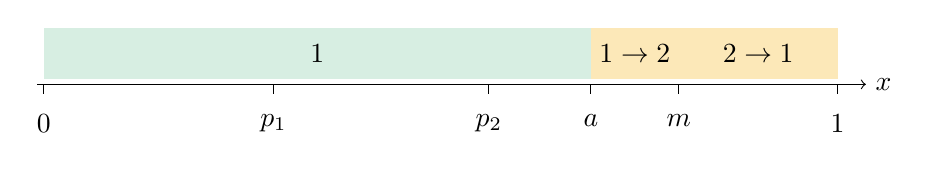
\begin{tikzpicture}[x=0.72cm,y=1cm]
    \definecolor{policyHold}{HTML}{D7EEE2}
    \definecolor{policyLow}{HTML}{FCE8B8}
    \fill[policyHold] (0,0.07) rectangle (9.65,0.72);
    \fill[policyLow] (9.65,0.07) rectangle (11.2,0.72);
    \fill[policyLow] (11.2,0.07) rectangle (14,0.72);
    \node at (4.825,0.395) {$1$};
    \node at (10.425,0.395) {$1\to2$};
    \node at (12.6,0.395) {$2\to1$};
    \draw[->] (-0.12,0) -- (14.5,0) node[right] {$x$};
    \foreach \x/\lab in {0/0,4.05/p_1,7.85/p_2,9.65/a,11.2/m,14/1} {
        \draw (\x,0) -- (\x,-0.12);
        \node[below=4pt] at (\x,-0.12) {$\lab$};
    }
    \end{tikzpicture}
    \end{figure}
\end{frame}

\begin{frame}
    \frametitle{When $m>p_2$}
    When $a<p_2$
    \begin{itemize}
        \item We have $F'(x)>0$ on $(p_2,m)$, so the table allows crossing $1\to2$
        \item If $H$ wins at $p_2$ by a contradiction argument we get that product 2 is optimal to the right of $p_2$
    \end{itemize}
    \begin{figure}[H]
    \centering
    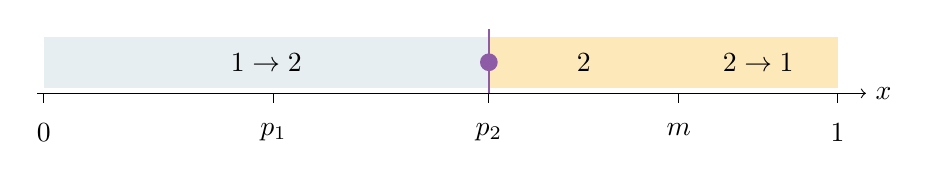
\begin{tikzpicture}[x=0.72cm,y=1cm]
    \definecolor{policyJoined}{HTML}{E7EEF2}
    \definecolor{policyLow}{HTML}{FCE8B8}
    \definecolor{policyBoundary}{HTML}{8E5BA6}
    \fill[policyJoined] (0,0.07) rectangle (7.85,0.72);
    \fill[policyLow] (7.85,0.07) rectangle (11.2,0.72);
    \fill[policyLow] (11.2,0.07) rectangle (14,0.72);
    \draw[policyBoundary,line width=0.8pt] (7.85,0) -- (7.85,0.82);
    \fill[policyBoundary] (7.85,0.395) circle (3.2pt);
    \node at (3.925,0.395) {$1\to2$};
    \node at (9.525,0.395) {$2$};
    \node at (12.6,0.395) {$2\to1$};
    \draw[->] (-0.12,0) -- (14.5,0) node[right] {$x$};
    \foreach \x/\lab in {0/0,4.05/p_1,7.85/p_2,11.2/m,14/1} {
        \draw (\x,0) -- (\x,-0.12);
        \node[below=4pt] at (\x,-0.12) {$\lab$};
    }
    \end{tikzpicture}
    \end{figure}

\end{frame}

\begin{frame}
    \frametitle{When $m>p_2$}
    When $a<p_2$
    \begin{itemize}
        \item Since all crossings inside $[p_1,p_2]$ have orientation $L \to H$, if $L$ wins at $p_2$ then $L$ wins throughout the interval 
        \item On $(p_2,m)$ we have $F'(x)>0$, so the table allows crossing $1\to2$
        \item On $(m,1)$ we have $F'(x)<0$, so the table allows crossing $2\to1$
        \item Then product 2 can be optimal on at most one interrval
    \end{itemize}
    \begin{figure}[H]
    \centering
    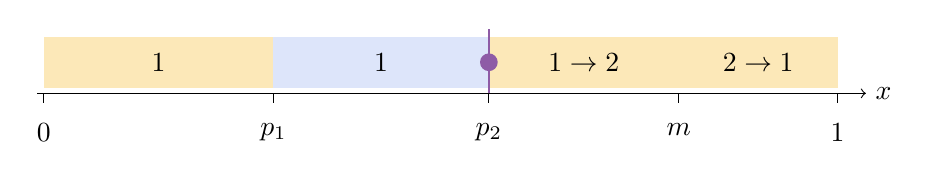
\begin{tikzpicture}[x=0.72cm,y=1cm]
    \definecolor{policyLow}{HTML}{FCE8B8}
    \definecolor{policyComparison}{HTML}{DDE5FA}
    \definecolor{policyBoundary}{HTML}{8E5BA6}
    \fill[policyLow] (0,0.07) rectangle (4.05,0.72);
    \fill[policyComparison] (4.05,0.07) rectangle (7.85,0.72);
    \fill[policyLow] (7.85,0.07) rectangle (11.2,0.72);
    \fill[policyLow] (11.2,0.07) rectangle (14,0.72);
    \draw[policyBoundary,line width=0.8pt] (7.85,0) -- (7.85,0.82);
    \fill[policyBoundary] (7.85,0.395) circle (3.2pt);
    \node at (2.025,0.395) {$1$};
    \node at (5.95,0.395) {$1$};
    \node at (9.525,0.395) {$1\to2$};
    \node at (12.6,0.395) {$2\to1$};
    \draw[->] (-0.12,0) -- (14.5,0) node[right] {$x$};
    \foreach \x/\lab in {0/0,4.05/p_1,7.85/p_2,11.2/m,14/1} {
        \draw (\x,0) -- (\x,-0.12);
        \node[below=4pt] at (\x,-0.12) {$\lab$};
    }
    \end{tikzpicture}
    \end{figure}

\end{frame}

\begin{frame}
    \frametitle{Endpoint ties}
    The crossing argument used before relies on $$W'(x) = \frac{g(x)}{b_i(x)}$$
    But at the endpoints we have 
    $$b_1(p_1)=0 \quad ,\quad b_2(p_2)=0$$
    so this argument cannot be applied directly. The goal then is to determine which product is optimal immediately on each side of the tie
\end{frame}

\begin{frame}
    \frametitle{Endpoint ties}
    \begin{itemize}
        \item At a tie at $p_1$, the policy switches from product 1 to product 2.
        \begin{center}
        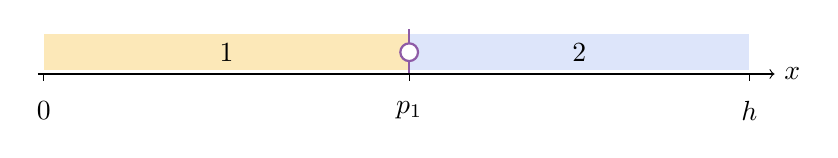
\begin{tikzpicture}[x=0.64cm,y=0.7cm]
        \definecolor{policyLow}{HTML}{FCE8B8}
        \definecolor{policyComparison}{HTML}{DDE5FA}
        \definecolor{policyBoundary}{HTML}{8E5BA6}
        \fill[policyLow] (0,0.07) rectangle (7.25,0.72);
        \fill[policyComparison] (7.25,0.07) rectangle (14,0.72);
        \draw[policyBoundary,line width=0.8pt] (7.25,0) -- (7.25,0.82);
        \draw[policyBoundary,fill=white,line width=0.8pt] (7.25,0.395) circle (3.2pt);
        \node at (3.625,0.395) {$1$};
        \node at (10.625,0.395) {$2$};
        \draw[->] (-0.12,0) -- (14.5,0) node[right] {$x$};
        \foreach \x/\lab in {0/0,7.25/p_1,14/h} {
            \draw (\x,0) -- (\x,-0.12);
            \node[below=4pt] at (\x,-0.12) {$\lab$};
        }
        \end{tikzpicture}
        \end{center}
        \item At a tie at $p_2$, the policy also switches from product 1 to product 2.
        \begin{center}
        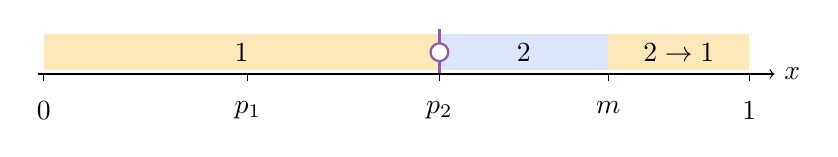
\begin{tikzpicture}[x=0.64cm,y=0.7cm]
        \definecolor{policyLow}{HTML}{FCE8B8}
        \definecolor{policyComparison}{HTML}{DDE5FA}
        \definecolor{policyBoundary}{HTML}{8E5BA6}
        \fill[policyLow] (0,0.07) rectangle (7.85,0.72);
        \fill[policyComparison] (7.85,0.07) rectangle (11.2,0.72);
        \fill[policyLow] (11.2,0.07) rectangle (14,0.72);
        \draw[policyBoundary,line width=0.8pt] (7.85,0) -- (7.85,0.82);
        \draw[policyBoundary,fill=white,line width=0.8pt] (7.85,0.395) circle (3.2pt);
        \node at (3.925,0.395) {$1$};
        \node at (9.525,0.395) {$2$};
        \node at (12.6,0.395) {$2\to1$};
        \draw[->] (-0.12,0) -- (14.5,0) node[right] {$x$};
        \foreach \x/\lab in {0/0,4.05/p_1,7.85/p_2,11.2/m,14/1} {
            \draw (\x,0) -- (\x,-0.12);
            \node[below=4pt] at (\x,-0.12) {$\lab$};
        }
        \end{tikzpicture}
        \end{center}
    \end{itemize}
\end{frame}

\begin{frame}
    \frametitle{With all this}
    \begin{itemize}
        \item All these arguments show that the only patterns that can occur are $1 \to 2$,  $2 \to 1$, $1 \to 2 \to 1$ and constant policies. Hence, the optimal policy uses product 2 at most one interval
        \item This proposition + the proof of existence of thresholds is the characterization that we can provide for the optimal policy
    \end{itemize}
    
\end{frame}




\end{document}
